\documentclass[a4paper,12pt]{article}

\usepackage[margin=1in]{geometry}
\usepackage{graphicx}
\usepackage{hyperref}
\usepackage{booktabs}%
\usepackage{xspace}
\usepackage{orcidlink}  % prettier orcid links
\usepackage{amsmath,amssymb,amsfonts}%
\usepackage{xcolor}%
\usepackage{xspace} 
\usepackage[labelformat=parens,labelsep=quad, skip=3pt]{caption}
\usepackage{siunitx}
\usepackage{comment}
\usepackage{array}
\usepackage{subcaption} % Added to support \captionsetup[subfigure]

\geometry{top=2cm,bottom=1in,left=1in,right=1in}

\usepackage[labelformat=parens,labelsep=quad, skip=3pt]{caption}
\captionsetup[subfigure]{labelfont=bf,singlelinecheck=off,justification=raggedright,labelformat=simple}


\usepackage[nolist]{acronym}

% Define acronyms
\begin{acronym}
\acro{AI}{Artificial Intelligence}
\acro{ANN}{Artificial Neural Networks}
\acro{AUC}{Area Under Curve }
\acro{CALD}{culturally and linguistically diverse}
\acro{CEDRIC}{The Comprehensive Epidemiological Database for Research, Innovation and Collaboration}
\acro{CNN}{Convolutional Neural Networks}
\acro{ED}{Emergency Department}
\acro{EHR}{Electronic Health Record}
\acro{ML}{Machine Learning}
\acro{NLP}{Nature Language Processing}
\acro{LLM}{Large Language Model}
\acro{ROC}{Receiver Operating Characteristic}
\acro{SDOH}{Social Determinants of Health}
\acro{SWERI}{South Western Emergency Research Institute}
\acro{SWSLHD}{South West Sydney Local Health District}
\acro{MIMIC}{Medical Information Mart for Intensive Care}
\acro{NSW}{New South Wales}
\acro{BERT}{Bidirectional Encoder Representations from Transformers}
\acro{NIH}{National Institutes of Health}
\acro{BCB}{Bio-Clinical BERT} 
\acro{CH}{Classification Head}
% \acro{Adam}{Adaptive Moment Estimation}
% \acro{AdamW}{Adaptive Moment Estimation with Decoupled Weight Decay Regularization}
% \acro{SGD}{Stochastic Gradient Descent}
\acro{NN}{Neural Network}
\acro{NN1}{Neural Network 1}
\acro{NN2}{Neural Network 2}
\acro{NN3}{Neural Network 3}
\acro{DS1}{Dataset 1: MIMIC-III Train Dataset}
\acro{HPC}{High Performance Computing}
\acro{MVA}{Motor Vehicle Accident}
\acro{BCBC}{Bio-Clinical BERT Classifier}
\acro{REGEX}{Regular Expression}
\acro{HREC}{Human Research Ethics Committee}
% Add more acronyms as needed
\end{acronym}


\newcommand{\figwidthf}{0.90\textwidth}
\newcommand{\figwidthh}{0.48\textwidth}
\newcommand{\figwidtht}{0.32\textwidth}
\newcommand{\figwidthhh}{0.45\textwidth}

\newcommand{\mimic}{\ac{MIMIC}-III\xspace}
\newcommand{\cedric}{\ac{CEDRIC}\xspace}   

% command for data sets
\newcommand{\mimicData}{MIMIC data\xspace}   % Note: This is the 2k MIMIC data that was labelled by Midhun
\newcommand{\inghamOne}{CEDRIC One\xspace}   % Note: this is the 1k Ingham data labelled by John 
\newcommand{\inghamTwo}{CEDRIC Two\xspace}  % Note: this is second set of 1k Ingham data labelled by Midhun and Jim

% table alignment
\newcolumntype{C}[1]{>{\centering\arraybackslash}p{#1}}


\title{Classification of kinetic-related injury in hospital triage data using NLP\\
-- \\
Supplementary Material}
\author{Midhun Shyam\orcidlink{0009-0006-2930-2135} \and
Jim Basilakis\orcidlink{0000-0002-7440-1320} \and
Kieran Luken\orcidlink{0000-0002-6147-693X} \and
Steven Thomas\orcidlink{0000-0002-2416-0020} \and
John Crozier\orcidlink{0000-0002-4773-8518} \and
Paul M Middleton\orcidlink{0000-0003-0760-1098} \and
X. Rosalind Wang\orcidlink{0000-0001-5454-6197}}

\date{}
% \author{redacted}
% \date{\today}

\begin{document}

\maketitle

%-------------------------------------------------------------------------------
% SECTION 1
%-------------------------------------------------------------------------------
\section{Data and Preprocessing}


We used data from two sources: \ac{MIMIC}-III and \cedric: 


\subsection{\ac{MIMIC}-III data}

The \mimic Clinical Database~\cite{johnson2016mimic3db}, publicly available through PhysioNet\footnote{a research resource founded in 1999 under the \ac{NIH}}~\cite{goldberger2000physiobank} provides free access to extensive physiological and clinical data alongside open-source software. The data comprises observations with presenting problems of over 40,000 critical care patients at the Beth Israel Deaconess Medical Center, Boston, Massachusetts \ac{ED}, between 2001 and 2012. 
We used the data collected from the critical care unit, specifically the table \texttt{NOTEEVENTS} that contains various de-identified clinical notes, for this paper. These data contains over two million samples of clinical notes, medical reports and discharge summaries, and is the same data set that the \ac{BCB} was originally trained on~\cite{alsentzer2019publicly}. 

For this work, we focused only on the free text data contained within the \texttt{TEXT} column. The \texttt{TEXT} data contains a variety of notes, 
such as ``History of Present Illness'', ``Chief Complaint'', ``Admit Diagnosis'' etc. For this work, only ``History of Present Illness'' notes were used, as it is most similar to triage notes. 
These notes were cleaned and truncated to 512 tokens, with encodings, special characters, empty lines, duplicates, recurring sentences within the same observation, and other irrelevant elements removed. This process reduced the dataset down to 
50,546 observations (henceforth called ``cleaned \texttt{NOTEEVENTS}''). Examples of critical care units clinical notes, similar to what is in this final set, are shown on the top table of Table~\ref{tab:exampleNotes}. 

We created a dataset --- henceforth called ``\emph{\mimicData}'' --- using the following steps: First, we used \ac{REGEX} to identify any notes in the cleaned \texttt{NOTEEVENTS} data related to positive cases that contain keywords specific to kinetic energy-related vehicular injuries (as listed under ``Vehicle'' in Table~\ref{tab:regexTerms}). 
This step classified 2034 observations as positive kinetic injury cases and 48,512 as other. Second, the subset of 2034 true cases underwent manual review, which identified 
725 
false cases. These are notes which had one or more of the keywords in the text, but were not patient presentations due to kinetic-related vehicular injuries. 

Third, to create a balanced dataset of equal numbers of positive and negative cases, we then added 583 notes to this data set, from the rest of the cleaned \texttt{NOTEEVENTS} data. 
These cases were randomly selected, but care was taken to ensure they followed the same word length distribution as the true cases. 
These samples also underwent manual review, where 176 were identified as possible true cases  and were thus excluded. 
Therefore, we created a dataset of 1309 positive kinetic-related vehicular injury cases and 1132 negative cases. 

    
\begin{table}[bt]
    \caption{Example of synthetic ICU (top) and triage (bottom) clinical notes for kinetic-related vehicular trauma cases (+ve label) and otherwise (-ve label). The corresponding rows in the tables show the exact same case, as would have been written by the two different departments. }
    \label{tab:exampleNotes}
    
    \begin{tabular}{@{}C{1.2cm} p{14cm}@{}}
    \toprule
    \textbf{Label} & 
    \multicolumn{1}{c}{\textbf{Example ICU clinical notes (similar to \mimicData)}} \\
    \midrule
    +ve & \scriptsize X, a 36-year-old marketing executive, was brought to the emergency department at 7:45 PM following a collision with a power pole while riding her electric bike. Witnesses reported she was travelling at approximately 30 km/h when she swerved to avoid a pedestrian and struck the pole chest-first. Upon arrival, she was conscious and oriented but visibly distressed, with vital signs showing tachycardia (HR 118), tachypnoea (RR 24), normal blood pressure (BP 112/74), and oxygen saturation of 97\% on room air. She complained of severe central chest pain radiating to her back, rating it 8/10, which worsened with inspiration. Primary survey revealed intact airway and breathing with no obvious external chest injuries, though auscultation noted muffled heart sounds. She was immediately transferred to the resuscitation bay where an eFAST scan revealed a significant pericardial effusion suggestive of cardiac tamponade. Urgent CT confirmed a moderate-sized pericardial effusion (2.3cm) with associated findings of cardiac compression. No aortic injury was identified, but a small right haemothorax was noted.  
    \par
    Upon return to the resuscitation bay,  \ldots\\
    -ve & \scriptsize An 80-year-old man, Mr. X, presented to the emergency department at 7:30 PM with confusion, fever, and severe lower abdominal pain. His daughter reported that he had been increasingly lethargic over the past 48 hours, with decreased oral intake and had become confused this evening. She noted he had complained of burning during urination for approximately three days but had refused to see his doctor.
    \par
    On examination, Mr. X was disoriented (Glasgow Coma Scale 13/15), febrile (temperature 39.2$^{\circ}C$), tachycardic (heart rate 118 bpm), hypotensive (BP 82/45 mmHg), and tachypnoeic (respiratory rate 28/min). He appeared pale and diaphoretic with delayed capillary refill of 4 seconds. His oxygen saturation was 94\% on room air.
    \par 
    \ldots
  \\
    \bottomrule
    \end{tabular}
    \vspace{2mm}
    
    \begin{tabular}{@{}C{1.2cm} p{14cm}@{}}
    \toprule
    \textbf{Label} & 
    \multicolumn{1}{c}{\textbf{Example triage notes (similar to \cedric Data)}} \\
    \midrule
    +ve & \scriptsize 36yo female presents post electric bike vs. power pole collision approx. 30 minutes ago. Alert but anxious, reports severe central chest pain 8/10, worse on inspiration. Denies LOC at scene. No helmet worn. O/E RR 24, SpO2 97\% RA, HR 118, BP 112/74, Temp 36.7°C. Skin clammy. No visible chest wall deformity but reporting pain on palpation of sternum. Multiple abrasions to right arm and leg. Known allergies to penicillin (rash). Not pregnant. No regular medications. \\
    -ve & \scriptsize 88yo man brought in by family, c/o abdominal pain, fever and suprapubic pain. Daughter also states that her father has been complaining for burning when he passes urine. PMHx of prostatism, hypertension, and T2DM. O/E Pale and sweaty, RR 28, SpO2 94\% RA, temp 39.2$^{\circ}$C, HR 118 bpm, BP 82/45, GCS 13/15. Confused and disorientated in time, place and person.   \\
    \bottomrule
    \end{tabular}
\vspace{-6mm}
\end{table}



\begin{table}[btp]
    \caption{Terms used in \ac{REGEX} pattern matching search. The terms identified for `vehicle' are those where possible kinetic injury took place. These terms are used to find the positive data in both databases. The terms identified for `trauma' are general trauma cases that are not specific to kinetic impact; these terms are only used to find non-kinetic related cases in the \cedric database. }
    \label{tab:regexTerms}
    \begin{tabular}{@{}l p{14cm}@{}}
    \toprule
    \textbf{Label} & \textbf{Terms used in \texttt{regex} text matching} \\
    \midrule
    Vehicle & \scriptsize mva, mba, vehicle, bus, pedestrian, passenger, ute, ped, bike, dirtbike, motorbike, pushbike, scooter, truck, bicycle, motorcycle, driver, driving, rtc, rta, \verb|\d*km[a-zA-Z/]*|, skateboard, surfing, surf, horse, collision, crossing, buggy, ebike, jetski, vs car, car vs, car accident, moving car, traffic light, traffic lights, hit by car, hit by a car, car hit, airbag, airbags, T boned, reversed, struck by car, struck by a car, tyre \\
    Trauma & \scriptsize \verb|(?<!nil )|trauma, \verb|(?<!nil )|injury, \verb|(?<!nil )|injured, \verb|(?<!nil )|injuries, strain, rupture, sprain, fracture, dislocation, damage, contusion, tear, assault, accident, homicide, blast, split, bruised, laceration, concussion, lac, crush, broken, fall, fallen, \# \\
    \bottomrule
    \end{tabular}
\vspace{-6mm}
\end{table}



\subsection{\cedric data}

%% -- Info below redacted for review purpose. 
\acf{CEDRIC} database is held at \ac{SWERI} within the Ingham Institute of Applied Medical Research, 
%\footnote{\url{https://sweri.com.au/}}
%\footnote{\url{https://inghaminstitute.org.au}}
it captures and links data from 
\ac{ED} presentations in \ac{SWSLHD}\footnote{Comprised of: Bankstown-Lidcombe, Bowral, Camden and Campbelltown, Fairfield, and Liverpool Hospitals.} 
since 2005. 

For this work, we concentrated on the \ac{ED} triage comments in \cedric (See bottom table of Table~\ref{tab:exampleNotes} for example triage notes). We performed a \ac{REGEX} word search of the database using the expressions listed in Table~\ref{tab:regexTerms} for positive and negative samples. To avoid duplicates in search results, we searched for samples in the different cases from two different years in the database. Furthermore, as we know that \ac{REGEX} will return a small percentage of false positive samples, and the number of negative samples greatly outnumbers positive samples in the database, we used terms from both cases to search for notes in the second year. To ensure we obtained a balanced data set, we returned the same number of samples from the two years in the database. Both data sets were manually inspected and labelled. 

We thus created two data sets: 
\vspace{-2mm}
\begin{enumerate}
    \item \inghamOne : positive cases from 2022 and both cases from 2021, resulting in 447 kinetic injury cases and 553 others. 
    \item \inghamTwo : positive cases from 2023 and both cases from 2022, resulting in 413 kinetic injury cases and 587 others. 
\end{enumerate}





%-------------------------------------------------------------------------------
% SECTION 2
%-------------------------------------------------------------------------------


\section{Fine-tuning on MIMIC data}

The results after fine-tuning the \ac{BCBC} configurations using the \ac{NN1}, \ac{NN2}, and \ac{NN3} fine-tuning strategies for the AdamW optimiser are presented in Figure~\ref{fig:res_training}, with Figure~\ref{fig:res_training}a. showing the accuracy, Figure~\ref{fig:res_training}b. showing the F1-Score, and Figure~\ref{fig:res_training}c. showing the total training time. Tables~\ref{tab:res_train_accuracy}, \ref{tab:res_train_f1score}, and \ref{tab:res_train_time} demonstrate the training accuracy, F1-score, and total training time (min) respectively for the \ac{NN3} architecture\footnote{Plots for \ac{NN1} and \ac{NN2} are presented in Supplementary Materials, which is in the GitHub repository, but omitted here for brevity given the overall results plotted in Figure~\ref{fig:res_training} and the similarity between \ac{NN} architectures. Similarly, tables for Adam and SGD optimisers are also in Supplementary Materials}. 

Figure~\ref{fig:res_training} demonstrates the different error metrics tested across each \ac{NN} architecture. We found that most learning/dropout rate combinations provided similar 
results, with the exception of the \ac{NN3} configuration using $lr = 0.005$, which had a significantly worse accuracy and F1-score. Excluding the models optimised using SGD, and the largest learning rate ($lr = 0.005$), the \ac{NN1} architecture performed worst across all metrics, with \ac{NN2} and \ac{NN3} performing similarly. We found that \ac{NN3} architecture, using the Adam optimiser with $lr = 0.0001$ and $dr = 0.15$ provided the best error metrics (accuracy of $95.0 \pm 0.9 \%$, and F1-score of $95.4 \pm 0.8\%$). However, this was at the expense of training time, as the AdamW optimiser was consistently quicker, with training times generally taking between a third and half as long as the Adam optimiser (Table~\ref{tab:res_train_time}), for marginally worse accuracy and F1-score. 


We performed a two-sampled t-test ($N=10$ for the number of repetitions of each model configurations trained) of all pairs of results in Tables~\ref{tab:res_train_accuracy} and \ref{tab:res_train_f1score} ten times. We observed that about half of the more than 300 pairs had statistically significant differences between the results at $p = 0.05$. The distinction between significant and non-significant difference was subtle --- e.g.\ $0.945 \pm 0.008$ vs.\ $0.933 \pm 0.010$ was not significant, while $0.947 \pm 0.013$ vs.\ $0.933 \pm 0.010$ was significant at $p = 0.05$. 
However, in a practical sense, there was no real difference between accuracies of $95.0 \pm 0.9\%$ (the best Adam configuration) and $94.2 \pm 1.2\%$ (the worst AdamW configuration, shown in Table~\ref{tab:res_train_accuracy}.) even though they were statistically significantly different. 


% Results using NN1
\begin{table}[h!]
	\caption{
	Accuracy, F1-score and training time on GPU of fine-tuning on MIMIC data with the different optimiser using NN1, 
	and at different learning and drop out rates.}
	\centering
		\resizebox{\textwidth}{!}{%
		\begin{tabular}{@{}lcccccc@{}}
		\toprule
		&  \multicolumn{6}{c}{Accuracy (Learning rate, Drop out rate)} \\ \cmidrule(l){2-7} 
		Optimiser & (0.0001, 0.15) & (0.0001, 0.2) & (0.0001, 0.25) & (0.0005, 0.15) & (0.0005, 0.2) & (0.0005, 0.25) \\ \midrule
		Adam & $0.902 \pm 0.011$ & $0.903 \pm 0.012$ & $0.903 \pm 0.012$ & $0.903 \pm 0.012$ & $0.903 \pm 0.011$ & $0.903 \pm 0.012$ \\
		AdamW & $0.902 \pm 0.013$ & $0.903 \pm 0.013$ & $0.904 \pm 0.012$ & $0.908 \pm 0.013$ & $0.908 \pm 0.011$ & $0.906 \pm 0.010$ \\
		SGD & $0.808 \pm 0.025$ & $0.816 \pm 0.023$ & $0.802 \pm 0.028$ & $0.872 \pm 0.013$ & $0.872 \pm 0.013$ & $0.872 \pm 0.010$ \\
				\bottomrule
		\end{tabular}
		}

	\resizebox{\textwidth}{!}{%
    \begin{tabular}{@{}lcccccc@{}}
    \toprule
    &  \multicolumn{6}{c}{F1-score (Learning rate, Drop out rate)} \\ \cmidrule(l){2-7} 
    Optimiser & (0.0001, 0.15) & (0.0001, 0.2) & (0.0001, 0.25) & (0.0005, 0.15) & (0.0005, 0.2) & (0.0005, 0.25) \\ \midrule
	Adam & $0.910 \pm 0.010$ & $0.911 \pm 0.011$ & $0.911 \pm 0.010$ & $0.912 \pm 0.011$ & $0.911 \pm 0.009$ & $0.911 \pm 0.011$ \\
	AdamW & $0.911 \pm 0.011$ & $0.912 \pm 0.011$ & $0.912 \pm 0.011$ & $0.915 \pm 0.011$ & $0.916 \pm 0.010$ & $0.914 \pm 0.009$ \\
	SGD & $0.838 \pm 0.020$ & $0.845 \pm 0.018$ & $0.835 \pm 0.022$ & $0.885 \pm 0.012$ & $0.884 \pm 0.011$ & $0.885 \pm 0.009$ \\
		\bottomrule
    \end{tabular}
	}

	\resizebox{\textwidth}{!}{%
    \begin{tabular}{@{}lcccccc@{}}
    \toprule
    &  \multicolumn{6}{c}{Time (Min) (Learning rate, Drop out rate)} \\ \cmidrule(l){2-7} 
	Adam & $52.012 \pm 31.871$ & $54.622 \pm 36.095$ & $53.690 \pm 33.143$ & $24.953 \pm 11.361$ & $28.247 \pm 13.267$ & $29.620 \pm 12.057$ \\
	AdamW & $60.175 \pm 36.935$ & $57.892 \pm 34.549$ & $58.152 \pm 35.111$ & $28.470 \pm 17.422$ & $30.002 \pm 21.738$ & $26.483 \pm 17.515$ \\
	SGD & $104.448 \pm 43.670$ & $104.433 \pm 43.664$ & $104.443 \pm 43.626$ & $94.610 \pm 40.999$ & $104.432 \pm 43.617$ & $103.918 \pm 43.134$ \\
		\bottomrule
    \end{tabular}
    }
	
\end{table}
	
% Results using NN2
\begin{table}[h!]
	\caption{Accuracy, F1-score and training time on GPU of fine-tuning on MIMIC data with the different optimiser using NN2, 
	and at different learning and drop out rates.}
	\centering
		\resizebox{\textwidth}{!}{%
		\begin{tabular}{@{}lcccccc@{}}
		\toprule
		&  \multicolumn{6}{c}{Accuracy (Learning rate, Drop out rate)} \\ \cmidrule(l){2-7} 
		Optimiser & (0.0001, 0.15) & (0.0001, 0.2) & (0.0001, 0.25) & (0.0005, 0.15) & (0.0005, 0.2) & (0.0005, 0.25) \\ \midrule
		Adam & $0.943 \pm 0.011$ & $0.944 \pm 0.010$ & $0.942 \pm 0.014$ & $0.943 \pm 0.015$ & $0.945 \pm 0.014$ & $0.942 \pm 0.012$ \\
		AdamW & $0.942 \pm 0.007$ & $0.945 \pm 0.009$ & $0.945 \pm 0.012$ & $0.945 \pm 0.010$ & $0.944 \pm 0.012$ & $0.944 \pm 0.006$ \\
		SGD & $0.852 \pm 0.021$ & $0.850 \pm 0.012$ & $0.846 \pm 0.019$ & $0.925 \pm 0.012$ & $0.920 \pm 0.013$ & $0.922 \pm 0.013$ \\
				\bottomrule
		\end{tabular}
		}

	\resizebox{\textwidth}{!}{%
    \begin{tabular}{@{}lcccccc@{}}
    \toprule
    &  \multicolumn{6}{c}{F1-score (Learning rate, Drop out rate)} \\ \cmidrule(l){2-7} 
    Optimiser & (0.0001, 0.15) & (0.0001, 0.2) & (0.0001, 0.25) & (0.0005, 0.15) & (0.0005, 0.2) & (0.0005, 0.25) \\ \midrule
	Adam & $0.947 \pm 0.010$ & $0.948 \pm 0.010$ & $0.946 \pm 0.013$ & $0.947 \pm 0.014$ & $0.949 \pm 0.013$ & $0.946 \pm 0.011$ \\
	AdamW & $0.946 \pm 0.007$ & $0.949 \pm 0.008$ & $0.949 \pm 0.011$ & $0.949 \pm 0.009$ & $0.948 \pm 0.012$ & $0.948 \pm 0.006$ \\
	SGD & $0.867 \pm 0.019$ & $0.865 \pm 0.012$ & $0.861 \pm 0.017$ & $0.932 \pm 0.011$ & $0.926 \pm 0.012$ & $0.929 \pm 0.011$ \\
		\bottomrule
    \end{tabular}
	}

	\resizebox{\textwidth}{!}{%
    \begin{tabular}{@{}lcccccc@{}}
    \toprule
    &  \multicolumn{6}{c}{Time (Min) (Learning rate, Drop out rate)} \\ \cmidrule(l){2-7} 
	Adam & $10.450 \pm 8.321$ & $8.648 \pm 2.085$ & $10.335 \pm 4.967$ & $7.272 \pm 2.570$ & $9.092 \pm 3.768$ & $11.217 \pm 3.999$ \\
	AdamW & $5.588 \pm 0.549$ & $6.293 \pm 2.313$ & $6.208 \pm 2.604$ & $6.108 \pm 2.612$ & $4.797 \pm 0.670$ & $5.293 \pm 1.869$ \\
	SGD & $106.710 \pm 44.473$ & $115.078 \pm 43.474$ & $106.702 \pm 44.418$ & $96.905 \pm 39.984$ & $85.037 \pm 39.787$ & $88.497 \pm 44.997$ \\
		\bottomrule
    \end{tabular}
    }
		
\end{table}

%% Table  NN3 results
\begin{table}[h!]
  \centering
  \caption{Results of fine-tuning \ac{NN3} using the different optimisers and at different hyperparameters. The best result for each optimiser is highlighted.} %For AdamW, the highlighted value has higher accuracy and F1-score in the fourth decimal place.}
  \label{tab:res_training}
  \begin{subtable}[t]{\textwidth}
    \centering
    \label{tab:res_train_accuracy}
  	\resizebox{\textwidth}{!}{%
    \begin{tabular}{@{}lcccccc@{}}
    \toprule
    &  \multicolumn{6}{c}{Accuracy (Learning rate, Drop out rate)} \\ \cmidrule(l){2-7} 
    Optimiser & (0.0001, 0.15) & (0.0001, 0.2) & (0.0001, 0.25) & (0.0005, 0.15) & (0.0005, 0.2) & (0.0005, 0.25) \\ \midrule
    Adam & \textbf{0.950 $\pm$ 0.009} & $0.948 \pm 0.009$ & $0.949 \pm 0.010$ & $0.948 \pm 0.011$ & $0.947 \pm 0.013$ & $0.944 \pm 0.009$ \\
    AdamW & $0.942 \pm 0.012$ & $0.947 \pm 0.008$ & $0.947 \pm 0.010$ & $0.946 \pm 0.010$ & \textbf{0.947 $\pm$ 0.009} & $0.945 \pm 0.008$ \\
    SGD & $0.899 \pm 0.022$ & $0.881 \pm 0.030$ & $0.908 \pm 0.021$ & $0.932 \pm 0.015$ & \textbf{0.937 $\pm$ 0.017} & $0.933 \pm 0.010$ \\
    \bottomrule
        \end{tabular}
  }  
  \end{subtable}
  
  \begin{subtable}[t]{\textwidth}
    \centering
    \label{tab:res_train_f1score}
	\resizebox{\textwidth}{!}{%
    \begin{tabular}{@{}lcccccc@{}}
    \toprule
    &  \multicolumn{6}{c}{F1-score (Learning rate, Drop out rate)} \\ \cmidrule(l){2-7} 
    Optimiser & (0.0001, 0.15) & (0.0001, 0.2) & (0.0001, 0.25) & (0.0005, 0.15) & (0.0005, 0.2) & (0.0005, 0.25) \\ \midrule
    Adam & \textbf{0.954 $\pm$ 0.008} & $0.952 \pm 0.008$ & $0.953 \pm 0.010$ & $0.951 \pm 0.010$ & $0.950 \pm 0.012$ & $0.948 \pm 0.009$ \\
    AdamW & $0.946 \pm 0.011$ & $0.951 \pm 0.008$ & $0.950 \pm 0.010$ & $0.950 \pm 0.009$ & \textbf{0.951 $\pm$ 0.008} & $0.949 \pm 0.008$ \\
    SGD & $0.908 \pm 0.018$ & $0.894 \pm 0.023$ & $0.916 \pm 0.017$ & $0.938 \pm 0.013$ & \textbf{0.942 $\pm$ 0.015} & $0.939 \pm 0.009$ \\
        \bottomrule
    \end{tabular}
    }
  \end{subtable}
  
  \begin{subtable}[t]{\textwidth}
    \centering
    \label{tab:res_train_time}
	\resizebox{\textwidth}{!}{%
    \begin{tabular}{@{}lcccccc@{}}
    \toprule
    &  \multicolumn{6}{c}{Time (min) (Learning rate, Drop out rate)} \\ \cmidrule(l){2-7} 
    Optimiser & (0.0001, 0.15) & (0.0001, 0.2) & (0.0001, 0.25) & (0.0005, 0.15) & (0.0005, 0.2) & (0.0005, 0.25) \\ \midrule
Adam & $11.267 \pm 7.288$ & $10.760 \pm 4.515$ & $10.070 \pm 3.622$ & \textbf{8.022 $\pm$ 3.161} & $9.663 \pm 4.318$ & $11.598 \pm 5.960$ \\
AdamW & \textbf{5.057 $\pm$ 0.505} & $5.905 \pm 2.276$ & $6.430 \pm 2.689$ & $6.327 \pm 3.350$ & $6.372 \pm 3.175$ & $5.898 \pm 2.603$ \\
SGD & $100.635 \pm 44.524$ & $100.660 \pm 44.502$ & $109.112 \pm 45.218$ & \textbf{76.850 $\pm$ 42.045} & $88.600 \pm 38.255$ & $77.797 \pm 53.375$ \\    
    \bottomrule
    \end{tabular}
    }
  \end{subtable}
  
\end{table}


%% Plots of AdamW results 
\begin{figure}[p] 
	\begin{center}
		\begin{subfigure}[b]{\figwidthh}
			\caption{} 
			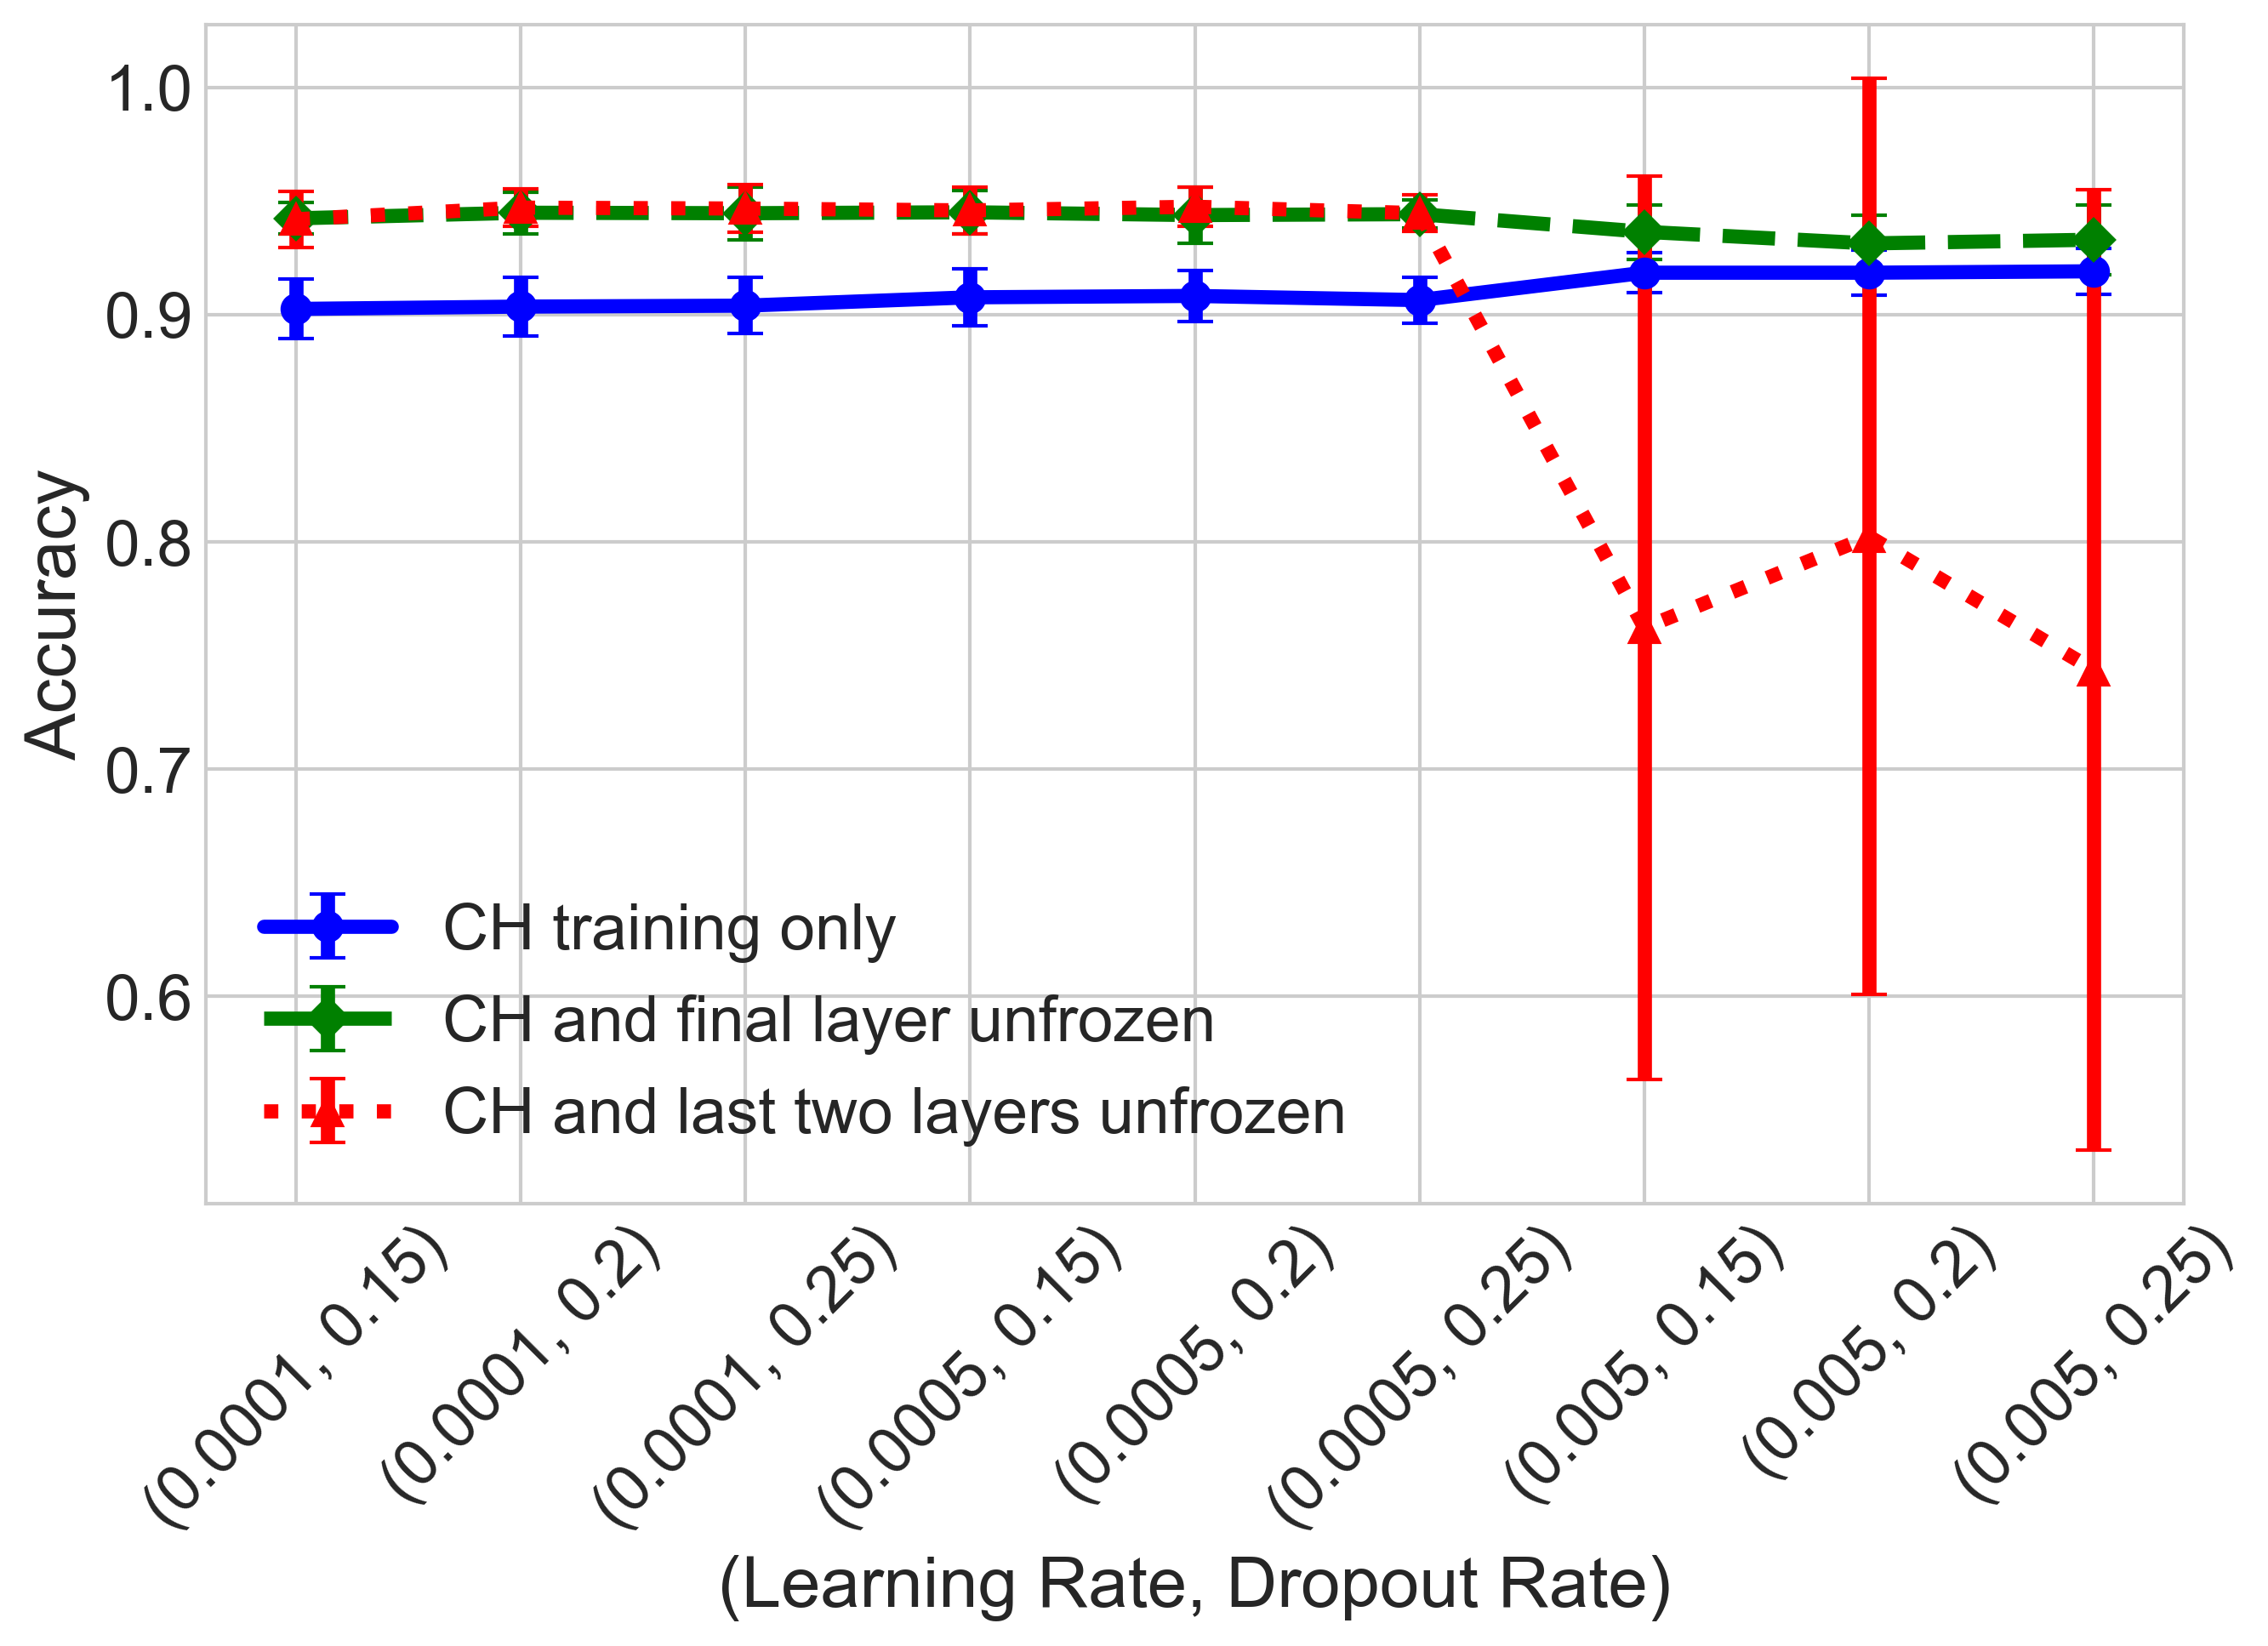
\includegraphics[width=\textwidth]{AdamW_optimiser_accuracy.png}
		\end{subfigure}
        \hfill
		\begin{subfigure}[b]{\figwidthh}
			\caption{}
			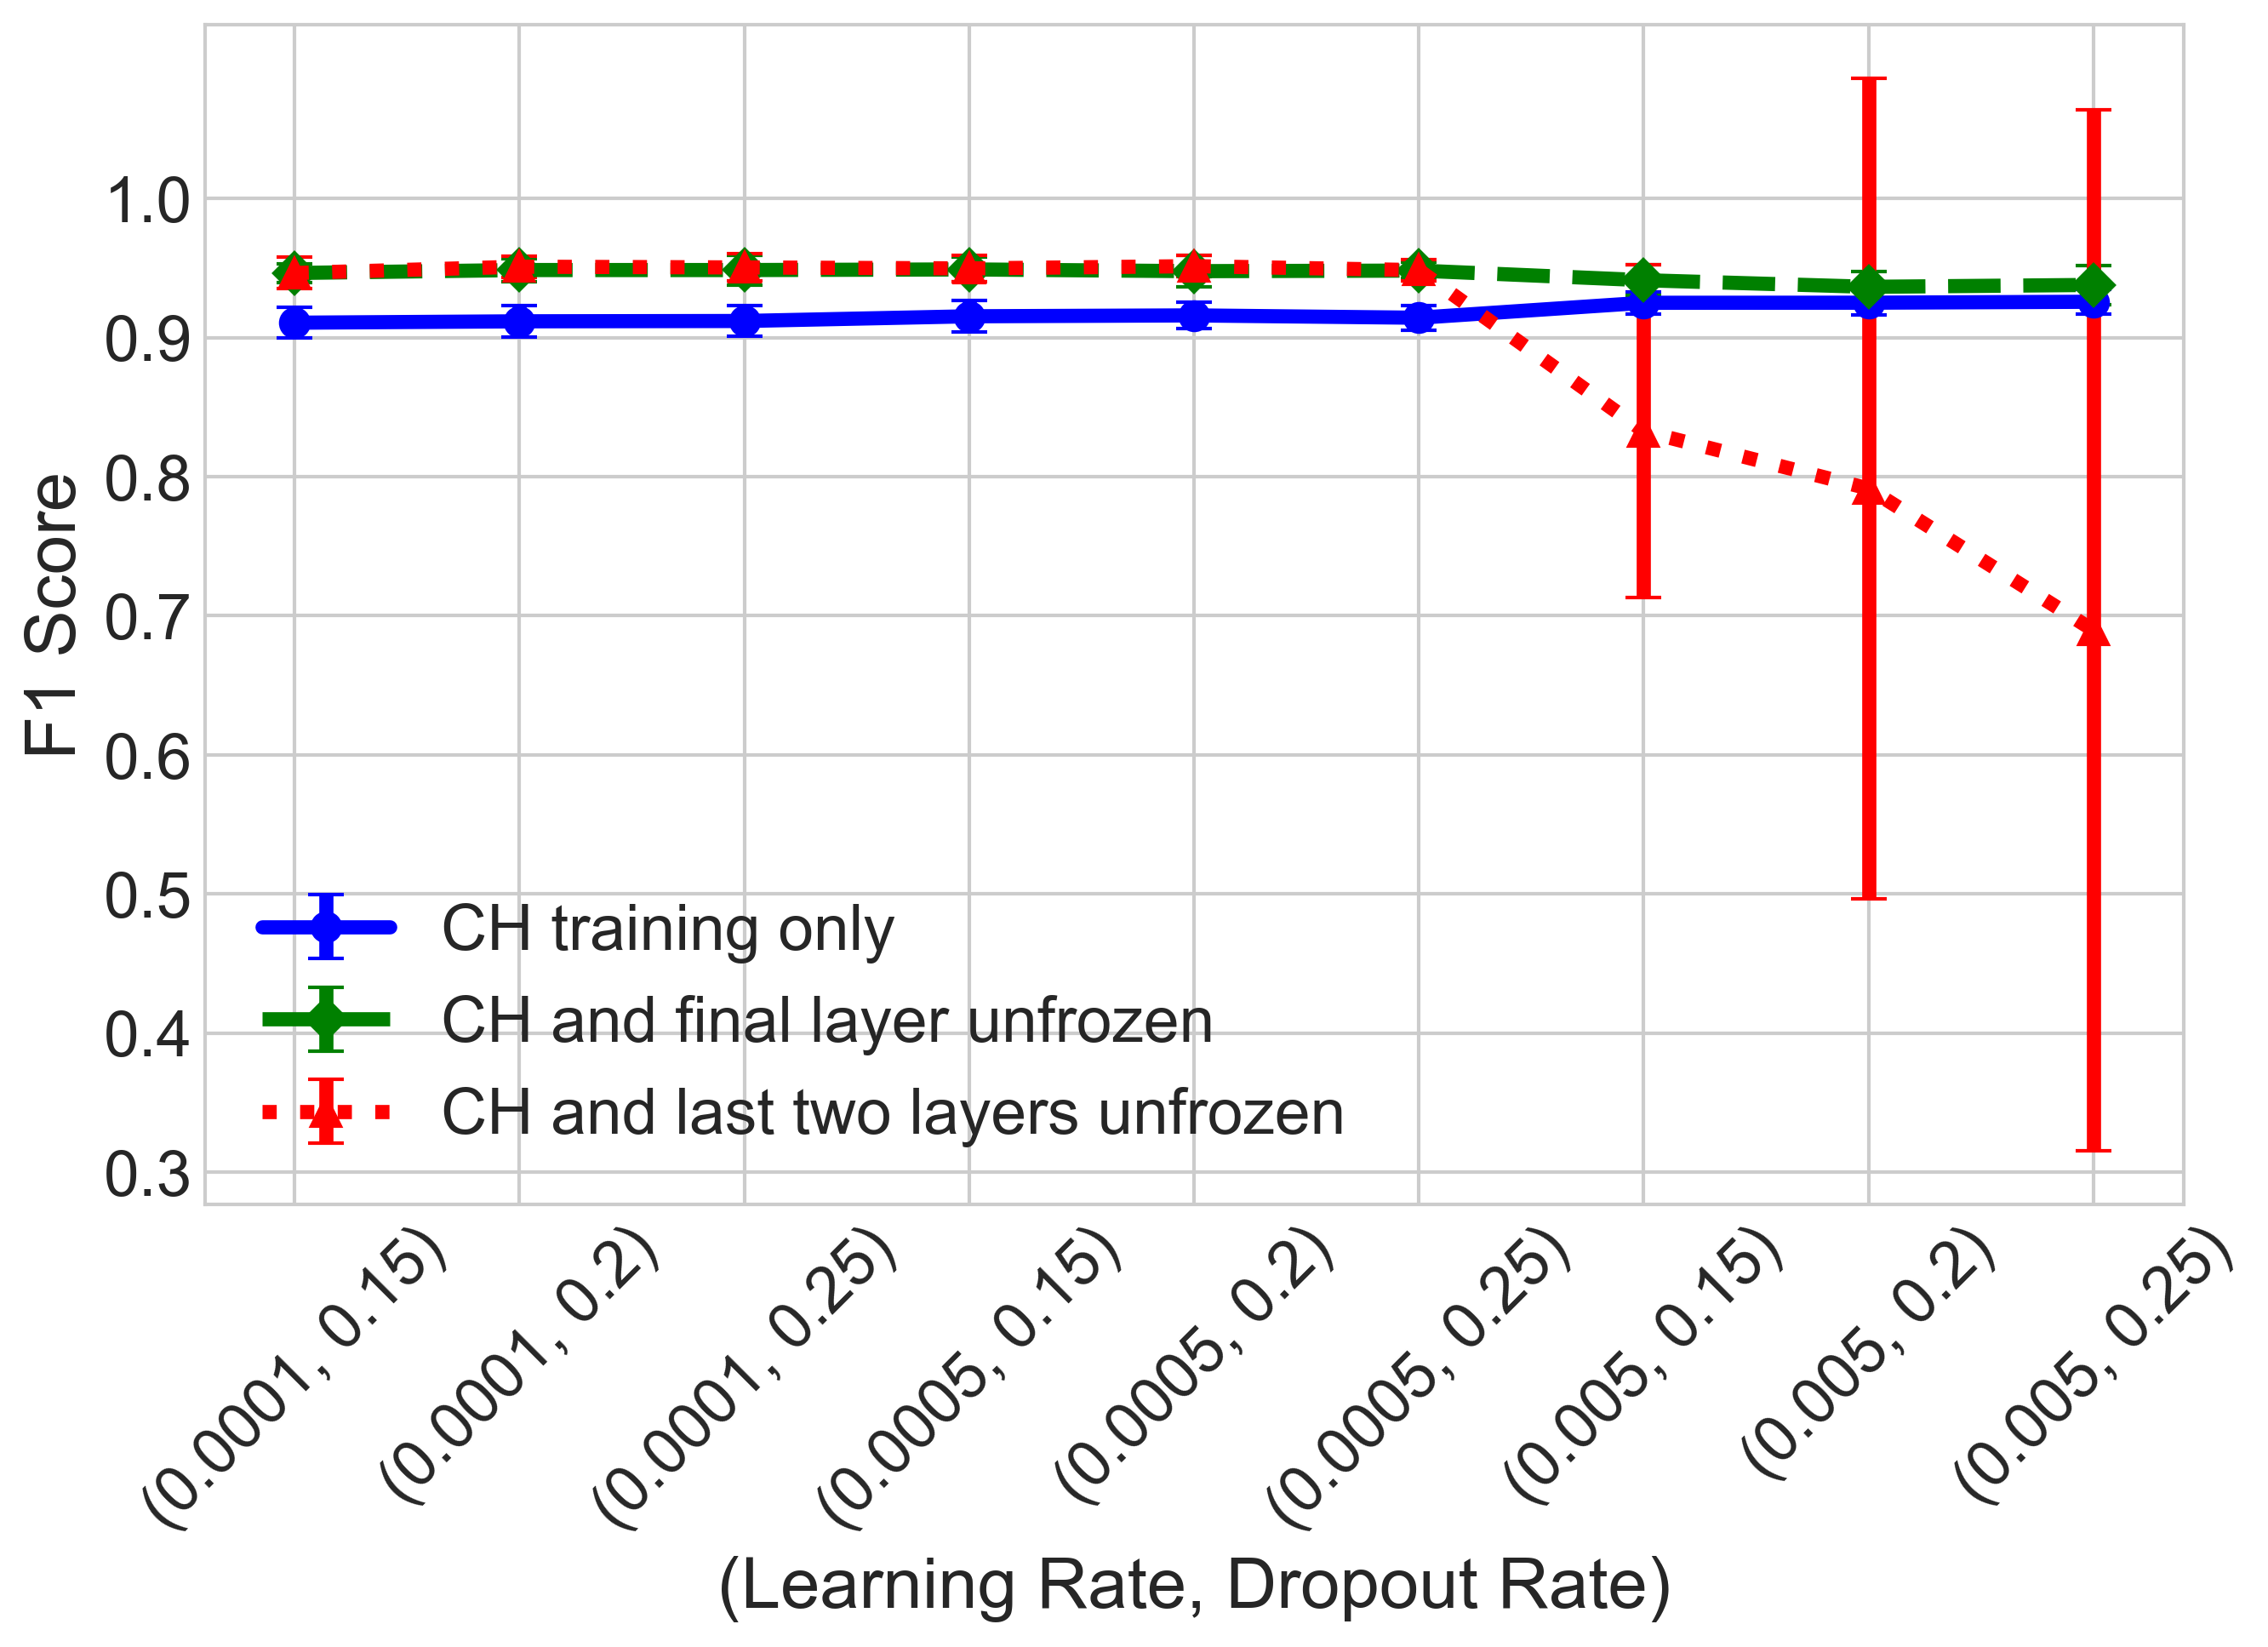
\includegraphics[width=\textwidth]{AdamW_optimiser_f1_score.png}
		\end{subfigure}
        \hfill
		\begin{subfigure}[b]{\figwidthh}
			\caption{}
			\includegraphics[width=\textwidth]{training_AdamW_optimiser_TrainingTimeMin.png}
		\end{subfigure}
	\end{center}
	\caption{Results of fine-tuning using the AdamW optimiser: (a) Accuracy of the validation data; (b) F-1 score on the validation data; (c) training time. 
	} 
	\label{fig:res_training}
\end{figure}

% Plots of Adam results
\begin{figure}[p] 
	\begin{center}
		\begin{subfigure}[b]{\figwidthh}
			\caption{} 
			\includegraphics[width=\textwidth]{training_Adam_optimiser_accuracy.png}
		\end{subfigure}
        \hfill
		\begin{subfigure}[b]{\figwidthh}
			\caption{}
			\includegraphics[width=\textwidth]{training_Adam_optimiser_f1_score.png}
		\end{subfigure}
        \hfill
		\begin{subfigure}[b]{\figwidthh}
			\caption{}
			\includegraphics[width=\textwidth]{training_Adam_optimiser_TrainingTimeMin.png}
		\end{subfigure}
	\end{center}
	\caption{Results of fine-tuning using the Adam optimiser: (a) Accuracy of the validation data; (b) F-1 score on the validation data; (c) training time. 
	} 
	\label{fig:res_training_adam}
\end{figure}

% Plots of SGD results
\begin{figure}[p] 
	\begin{center}
		\begin{subfigure}[b]{\figwidthh}
			\caption{} 
			\includegraphics[width=\textwidth]{training_SGD_optimiser_accuracy.png}
		\end{subfigure}
        \hfill
		\begin{subfigure}[b]{\figwidthh}
			\caption{}
			\includegraphics[width=\textwidth]{training_SGD_optimiser_f1_score.png}
		\end{subfigure}
        \hfill
		\begin{subfigure}[b]{\figwidthh}
			\caption{}
			\includegraphics[width=\textwidth]{training_SGD_optimiser_TrainingTimeMin.png}
		\end{subfigure}
	\end{center}
	\caption{Results of fine-tuning using the SGD optimiser: (a) Accuracy of the validation data; (b) F-1 score on the validation data; (c) training time. 
	} 
	\label{fig:res_training_SGD}
\end{figure}





    


\clearpage

\newpage

%-------------------------------------------------------------------------------
% SECTION 3
%-------------------------------------------------------------------------------


\section{Prediction with fine-tuned models}


The prediction results from the fine-tuned models are presented in Figure~\ref{fig:res_predict1} and Table~\ref{tab:res_prediction1}. We found that the results mirror those in Section~\ref{sec:finetune_mimic}, with the Adam and AdamW optimised models providing roughly the same accuracies and F1-scores. Like Section~\ref{sec:finetune_mimic}, the SGD optimised models, and $lr = 0.005$ perform the worst. 

We found the model that provides the best accuracy and F1-score is the AdamW optimised \ac{NN3} architecture, using $lr = 0.0005$ and $dr = 0.15$ --- a similar configuration to Section~\ref{sec:finetune_mimic} --- giving an accuracy of $83.9 \pm 1.8\%$, and an F1-score of $80 \pm 2.5\%$. Similar to Section~\ref{sec:finetune_mimic}, about half of the accuracy and F1-score pairs reported exhibited a statistically significantly difference between the results at $p = 0.05$. However, as noted in Section~\ref{sec:finetune_mimic}, the practical difference for clinicians between a model producing an accuracy of 83.9\% (AdamW optimised \ac{NN3} with $lr = 0.0005$ and $dr = 0.15$) and another with an accuracy of 82.0\% (AdamW optimised \ac{NN3} with $lr = 0.0001, dr = 0.15$) is minimal. 

% for accuracy: 
% -- 76 pairs > 0.05 
% -- 80 pairs > 0.001 
% for f1 score: 
% -- 71 pairs > 0.05
% -- 78 pairs > 0.001

We note that the drop in accuracy from $\sim95\%$ reported Section~\ref{sec:finetune_mimic} to $\sim84\%$ is not unexpected, as the fine-tuned model has been fine-tuned with data from one context (the \mimicData). This section then took those trained models, and tested them against the \inghamTwo data --- a fundamentally different context, as seen in Table~\ref{tab:exampleNotes}. 

The total prediction time as shown in Figure~\ref{fig:res_predict1}c was similar across all configurations, which is not surprising. All fine-tuned models took between 170 and 290 seconds to predict the data set of 1000 triage notes. Hence, this task could easily be achieved on much larger datasets within medical facilities. \ac{SWSLHD} receives around half a million patients in \ac{ED} in a year, this means even with minimum computing resources the classification process will take just one day for a year's data. 

Given the significant under-performance of the \ac{NN1} architecture, the SGD optimised models, and the models with a learning rate of 0.005, we did not continue further testing with these models. 




% NN1 results
\begin{table}[h!]
	\caption{Prediction results on \inghamTwo using fine-tuned NN1 with the different optimisers and at different learning and drop out rates. }
	\centering
		\resizebox{\textwidth}{!}{%
		\begin{tabular}{@{}lcccccc@{}}
		\toprule
		&  \multicolumn{6}{c}{Accuracy (Learning rate, Drop out rate)} \\ \cmidrule(l){2-7} 
		Optimiser & (0.0001, 0.15) & (0.0001, 0.2) & (0.0001, 0.25) & (0.0005, 0.15) & (0.0005, 0.2) & (0.0005, 0.25) \\ \midrule
		Adam & $0.672 \pm 0.008$ & $0.672 \pm 0.009$ & $0.673 \pm 0.007$ & $0.683 \pm 0.009$ & $0.682 \pm 0.004$ & $0.686 \pm 0.009$ \\
		AdamW & $0.675 \pm 0.015$ & $0.682 \pm 0.011$ & $0.682 \pm 0.010$ & $0.695 \pm 0.012$ & $0.696 \pm 0.010$ & $0.693 \pm 0.008$ \\
		SGD & $0.521 \pm 0.034$ & $0.516 \pm 0.024$ & $0.519 \pm 0.024$ & $0.598 \pm 0.012$ & $0.596 \pm 0.012$ & $0.599 \pm 0.016$ \\
						\bottomrule
		\end{tabular}
		}

	\resizebox{\textwidth}{!}{%
    \begin{tabular}{@{}lcccccc@{}}
    \toprule
    &  \multicolumn{6}{c}{F1-score (Learning rate, Drop out rate)} \\ \cmidrule(l){2-7} 
    Optimiser & (0.0001, 0.15) & (0.0001, 0.2) & (0.0001, 0.25) & (0.0005, 0.15) & (0.0005, 0.2) & (0.0005, 0.25) \\ \midrule
	Adam & $0.612 \pm 0.013$ & $0.612 \pm 0.015$ & $0.611 \pm 0.015$ & $0.628 \pm 0.010$ & $0.629 \pm 0.008$ & $0.630 \pm 0.011$ \\
	AdamW & $0.616 \pm 0.019$ & $0.622 \pm 0.012$ & $0.621 \pm 0.012$ & $0.641 \pm 0.010$ & $0.640 \pm 0.009$ & $0.636 \pm 0.009$ \\
	SGD & $0.561 \pm 0.032$ & $0.566 \pm 0.018$ & $0.558 \pm 0.045$ & $0.553 \pm 0.015$ & $0.543 \pm 0.020$ & $0.558 \pm 0.019$ \\
			\bottomrule
    \end{tabular}
	}

	% \resizebox{\textwidth}{!}{%
    % \begin{tabular}{@{}lcccccc@{}}
    % \toprule
    % &  \multicolumn{6}{c}{Time (Sec) (Learning rate, Drop out rate)} \\ \cmidrule(l){2-7} 
	% 	\bottomrule
    % \end{tabular}
    % }
	
\end{table}
	
% NN2 results
\begin{table}[h!]
	\caption{Prediction results on \inghamTwo using fine-tuned NN2 using the different optimisers and at different learning and drop out rates. }
	\centering
		\resizebox{\textwidth}{!}{%
		\begin{tabular}{@{}lcccccc@{}}
		\toprule
		&  \multicolumn{6}{c}{Accuracy (Learning rate, Drop out rate)} \\ \cmidrule(l){2-7} 
		Optimiser & (0.0001, 0.15) & (0.0001, 0.2) & (0.0001, 0.25) & (0.0005, 0.15) & (0.0005, 0.2) & (0.0005, 0.25) \\ \midrule
		Adam & $0.814 \pm 0.020$ & $0.818 \pm 0.010$ & $0.815 \pm 0.014$ & $0.818 \pm 0.016$ & $0.828 \pm 0.013$ & $0.824 \pm 0.014$ \\
		AdamW & $0.812 \pm 0.015$ & $0.820 \pm 0.013$ & $0.808 \pm 0.017$ & $0.828 \pm 0.010$ & $0.825 \pm 0.016$ & $0.818 \pm 0.014$ \\
		SGD & $0.596 \pm 0.028$ & $0.573 \pm 0.047$ & $0.593 \pm 0.031$ & $0.727 \pm 0.019$ & $0.722 \pm 0.026$ & $0.726 \pm 0.020$ \\
						\bottomrule
		\end{tabular}
		}

	\resizebox{\textwidth}{!}{%
    \begin{tabular}{@{}lcccccc@{}}
    \toprule
    &  \multicolumn{6}{c}{F1-score (Learning rate, Drop out rate)} \\ \cmidrule(l){2-7} 
    Optimiser & (0.0001, 0.15) & (0.0001, 0.2) & (0.0001, 0.25) & (0.0005, 0.15) & (0.0005, 0.2) & (0.0005, 0.25) \\ \midrule
	Adam & $0.756 \pm 0.019$ & $0.756 \pm 0.017$ & $0.756 \pm 0.019$ & $0.763 \pm 0.016$ & $0.775 \pm 0.021$ & $0.769 \pm 0.015$ \\
	AdamW & $0.762 \pm 0.014$ & $0.769 \pm 0.013$ & $0.761 \pm 0.011$ & $0.785 \pm 0.012$ & $0.781 \pm 0.020$ & $0.774 \pm 0.016$ \\
	SGD & $0.521 \pm 0.053$ & $0.547 \pm 0.049$ & $0.519 \pm 0.040$ & $0.686 \pm 0.020$ & $0.665 \pm 0.027$ & $0.677 \pm 0.013$ \\
			\bottomrule
    \end{tabular}
	}

	% \resizebox{\textwidth}{!}{%
    % \begin{tabular}{@{}lcccccc@{}}
    % \toprule
    % &  \multicolumn{6}{c}{Time (Min) (Learning rate, Drop out rate)} \\ \cmidrule(l){2-7} 
	% 	\bottomrule
    % \end{tabular}
    %}
		
\end{table}

%% Tables of accuracy and F1 score from prediction, NN3
\begin{table}[h!]
\caption{Accuracy and F1-score of prediction on \inghamTwo data using the fine-tuned \ac{NN3} models. 
The best result for each optimiser is highlighted. 
}
\label{tab:res_prediction1}
\centering
	\resizebox{\textwidth}{!}{%
    \begin{tabular}{@{}lcccccc@{}}
    \toprule
    &  \multicolumn{6}{c}{Accuracy (Learning rate, Drop out rate)} \\ \cmidrule(l){2-7} 
Optimiser & (0.0001, 0.15) & (0.0001, 0.2) & (0.0001, 0.25) & (0.0005, 0.15) & (0.0005, 0.2) & (0.0005, 0.25) \\ \midrule
Adam & $0.831 \pm 0.011$ & $0.832 \pm 0.010$ & \textbf{0.833 $\pm$ 0.012} & $0.832 \pm 0.015$ & $0.833 \pm 0.015$ & $0.826 \pm 0.021$ \\
AdamW & $0.820 \pm 0.016$ & $0.829 \pm 0.012$ & $0.820 \pm 0.012$ & \textbf{0.839 $\pm$ 0.018} & $0.828 \pm 0.017$ & $0.830 \pm 0.015$ \\
SGD & $0.657 \pm 0.056$ & $0.610 \pm 0.086$ & $0.671 \pm 0.051$ & $0.721 \pm 0.065$ & \textbf{0.735 $\pm $0.049} & $0.729 \pm 0.056$ \\
    \bottomrule
        \end{tabular}
    }
\vspace{2mm}

	\resizebox{\textwidth}{!}{%
    \begin{tabular}{@{}lcccccc@{}}
    \toprule
    &  \multicolumn{6}{c}{F1 Score (Learning rate, Drop out rate)} \\ \cmidrule(l){2-7} 
Optimiser & (0.0001, 0.15) & (0.0001, 0.2) & (0.0001, 0.25) & (0.0005, 0.15) & (0.0005, 0.2) & (0.0005, 0.25) \\ \midrule
Adam & $0.770 \pm 0.017$ & $0.769 \pm 0.020$ & \textbf{0.776 $\pm$ 0.022} & $0.774 \pm 0.026$ & $0.774 \pm 0.023$ & $0.763 \pm 0.036$ \\
AdamW & $0.777 \pm 0.017$ & $0.785 \pm 0.018$ & $0.773 \pm 0.018$ & \textbf{0.800 $\pm$ 0.025} & $0.788 \pm 0.020$ & $0.783 \pm 0.024$ \\
SGD & $0.615 \pm 0.025$ & $0.609 \pm 0.019$ & $0.619 \pm 0.020$ & $0.693 \pm 0.033$ & \textbf{0.702 $\pm$ 0.025} & $0.694 \pm 0.029$ \\
    \bottomrule
        \end{tabular}
    }

\end{table}


% Adam plots
\begin{figure}[p] 
	\begin{center}
		\begin{subfigure}[b]{\figwidthh}
			\caption{} 
			\includegraphics[width=\textwidth]{prediction_Adam_optimiser_accuracy.png}
		\end{subfigure}
        \hfill
		\begin{subfigure}[b]{\figwidthh}
			\caption{}
			\includegraphics[width=\textwidth]{prediction_Adam_optimiser_f1_score.png}
		\end{subfigure}
        \hfill
		\begin{subfigure}[b]{\figwidthh}
			\caption{}
			\includegraphics[width=\textwidth]{prediction_Adam_optimiser_PredictTimeSeconds.png}
		\end{subfigure}
	\end{center}
	\caption{Results of prediction on In-house Two using models fine-tuned with the Adam optimiser: 
	(a) Prediction accuracy; (b) F-1 score; (c) Prediction on CPU time (s).
	} 
	\label{fig:res_prdict_adam}
\end{figure}

% SGD plots
\begin{figure}[p] 
	\begin{center}
		\begin{subfigure}[b]{\figwidthh}
			\caption{} 
			\includegraphics[width=\textwidth]{prediction_SGD_optimiser_accuracy.png}
		\end{subfigure}
        \hfill
		\begin{subfigure}[b]{\figwidthh}
			\caption{}
			\includegraphics[width=\textwidth]{prediction_SGD_optimiser_f1_score.png}
		\end{subfigure}
        \hfill
		\begin{subfigure}[b]{\figwidthh}
			\caption{}
			\includegraphics[width=\textwidth]{prediction_SGD_optimiser_PredictTimeSeconds.png}
		\end{subfigure}
	\end{center}
	\caption{Results of prediction on In-house Two using models fine-tuned with the SGD optimiser: 
	(a) Prediction accuracy; (b) F-1 score; (c) Prediction on CPU time (s).
	} 
	\label{fig:res_predict_SGD}
\end{figure}

%% Plots for AdamW prediction results, step 2
\begin{figure}[p]
	\begin{center}
		\begin{subfigure}[b]{\figwidthh}
			\caption{} 
			\includegraphics[width=\textwidth]{prediction_AdamW_optimiser_accuracy.png}
		\end{subfigure}
        \hfill
		\begin{subfigure}[b]{\figwidthh}
			\caption{}
			\includegraphics[width=\textwidth]{prediction_AdamW_optimiser_f1_score.png}
		\end{subfigure}
        \hfill
		\begin{subfigure}[b]{\figwidthh}
			\caption{}
			\includegraphics[width=\textwidth]{prediction_AdamW_optimiser_PredictTimeSeconds.png}
		\end{subfigure}
	\end{center}
	\caption{Results of prediction on \inghamTwo using models fine-tuned with the AdamW optimiser: (a) Prediction accuracy; (b) F-1 score; (c) Prediction on CPU time (s). 
	} 
	\label{fig:res_predict1}
\end{figure}



\newpage


%-------------------------------------------------------------------------------
% SECTION 4
%-------------------------------------------------------------------------------

\section{Further fine-tuning on In-House One Data}

	
\begin{table}[h!]
	\caption{Accuracy, F1-score and training time on CPU of further fine-tuning (domain adaptation) on \inghamOne data with the different optimiser using NN2, 
	and at different learning and drop out rates.
	}
	\centering
		\resizebox{\textwidth}{!}{%
		\begin{tabular}{@{}lcccccc@{}}
		\toprule
		&  \multicolumn{6}{c}{Accuracy (Learning rate, Drop out rate)} \\ \cmidrule(l){2-7} 
	Optimiser & (0.0001, 0.15) & (0.0001, 0.2) & (0.0001, 0.25) & (0.0005, 0.15) & (0.0005, 0.2) & (0.0005, 0.25) \\ \midrule
	Adam & $0.936 \pm 0.008$ & $0.929 \pm 0.012$ & $0.928 \pm 0.011$ & $0.938 \pm 0.009$ & $0.943 \pm 0.011$ & $0.940 \pm 0.009$ \\
	AdamW & $0.923 \pm 0.011$ & $0.932 \pm 0.015$ & $0.922 \pm 0.013$ & $0.934 \pm 0.013$ & $0.941 \pm 0.013$ & $0.934 \pm 0.006$ \\
		\bottomrule
			\end{tabular}
		}
	
	\vspace{5mm}
		\resizebox{\textwidth}{!}{%
		\begin{tabular}{@{}lcccccc@{}}
		\toprule
		&  \multicolumn{6}{c}{F1 Score (Learning rate, Drop out rate)} \\ \cmidrule(l){2-7} 
	Optimiser & (0.0001, 0.15) & (0.0001, 0.2) & (0.0001, 0.25) & (0.0005, 0.15) & (0.0005, 0.2) & (0.0005, 0.25) \\ \midrule
	Adam & $0.930 \pm 0.009$ & $0.923 \pm 0.013$ & $0.922 \pm 0.011$ & $0.932 \pm 0.009$ & $0.937 \pm 0.013$ & $0.934 \pm 0.009$ \\
	AdamW & $0.916 \pm 0.011$ & $0.927 \pm 0.015$ & $0.916 \pm 0.014$ & $0.928 \pm 0.013$ & $0.936 \pm 0.014$ & $0.928 \pm 0.007$ \\
		\bottomrule
			\end{tabular}
		}
	\vspace{5mm}
	\resizebox{\textwidth}{!}{%
	\begin{tabular}{@{}lcccccc@{}}
	\toprule
	&  \multicolumn{6}{c}{Time (min) (Learning rate, Drop out rate)} \\ \cmidrule(l){2-7} 
Optimiser & (0.0001, 0.15) & (0.0001, 0.2) & (0.0001, 0.25) & (0.0005, 0.15) & (0.0005, 0.2) & (0.0005, 0.25) \\ \midrule
Adam & $198.092 \pm 59.439$ & $184.190 \pm 48.655$ & $185.488 \pm 45.923$ & $131.315 \pm 40.023$ & $127.185 \pm 63.776$ & $98.440 \pm 21.057$ \\
AdamW & $111.487 \pm 32.506$ & $104.337 \pm 24.244$ & $178.830 \pm 14.122$ & $166.618 \pm 32.676$ & $148.200 \pm 20.756$ & $93.328 \pm 21.506$ \\
	\bottomrule
		\end{tabular}
	}
	\end{table}
	
	
\begin{figure}[h!]
	\begin{center}
		\begin{subfigure}[b]{\figwidthhh}
			\caption{} 
			\includegraphics[width=\textwidth]{finetuning_Adam_optimiser_accuracy.png}
		\end{subfigure}
        \hfill
		\begin{subfigure}[b]{\figwidthhh}
			\caption{}
			\includegraphics[width=\textwidth]{finetuning_Adam_optimiser_f1_score.png}
		\end{subfigure}
        \hfill
		\begin{subfigure}[b]{\figwidthhh}
			\caption{}
			\includegraphics[width=\textwidth]{finetuning_Adam_optimiser_TrainingTimeMin.png}
		\end{subfigure}
	\end{center}                                                                
	\caption{Results of further fine-tuning on \inghamOne data with the Adam optimiser: (a) Prediction accuracy; (b) F-1 score; (c) Training time on CPU (min).
	} 
\end{figure}



%% Plots of AdamW results, step 3
\begin{figure}[tb]
	\begin{center}
		\begin{subfigure}[b]{\figwidtht}
			\caption{} 
			\includegraphics[width=\textwidth]{finetuning_AdamW_optimiser_accuracy.png}
		\end{subfigure}
        \hfill
		\begin{subfigure}[b]{\figwidtht}
			\caption{}
			\includegraphics[width=\textwidth]{finetuning_AdamW_optimiser_f1_score.png}
		\end{subfigure}
        \hfill
		\begin{subfigure}[b]{\figwidtht}
			\caption{}
			\includegraphics[width=\textwidth]{finetuning_AdamW_optimiser_TrainingTimeMin.png}
		\end{subfigure}
	\end{center}
	\caption{Results of further fine-tuning (domain adaptation) on \inghamOne data with the AdamW optimiser: (a) Prediction accuracy; (b) F-1 score; (c) Training time on CPU (min).
	} 
	\label{fig:res_domainAdaptation}
\end{figure}

%% Tables for NN3 step 3 -- accuracy, F1-score, time
\begin{table}[tb]
\caption{Accuracy, F1-score and training time on CPU of further fine-tuning on \inghamOne data with the AdamW optimiser using \ac{NN3}. 
The best result for each optimiser is highlighted. 
}
\label{tab:res_domainAdaptation}
\centering
	\resizebox{\textwidth}{!}{%
    \begin{tabular}{@{}lcccccc@{}}
    \toprule
    &  \multicolumn{6}{c}{Accuracy (Learning rate, Drop out rate)} \\ \cmidrule(l){2-7} 
Optimiser & (0.0001, 0.15) & (0.0001, 0.2) & (0.0001, 0.25) & (0.0005, 0.15) & (0.0005, 0.2) & (0.0005, 0.25) \\ \midrule
Adam & $0.945 \pm 0.011$ & $0.942 \pm 0.012$ & $0.940 \pm 0.009$ & $0.940 \pm 0.013$ & \textbf{0.945 $\pm$ 0.009} & $0.943 \pm 0.012$ \\
AdamW & $0.936 \pm 0.009$ & \textbf{0.945 $\pm$ 0.017} & $0.935 \pm 0.011$ & $0.938 \pm 0.011$ & $0.937 \pm 0.012$ & $0.936 \pm 0.011$ \\
    \bottomrule
        \end{tabular}
    }
\vspace{2mm}

	\resizebox{\textwidth}{!}{%
    \begin{tabular}{@{}lcccccc@{}}
    \toprule
    &  \multicolumn{6}{c}{F1 Score (Learning rate, Drop out rate)} \\ \cmidrule(l){2-7} 
Optimiser & (0.0001, 0.15) & (0.0001, 0.2) & (0.0001, 0.25) & (0.0005, 0.15) & (0.0005, 0.2) & (0.0005, 0.25) \\ \midrule
Adam & \textbf{0.940 $\pm$ 0.012} & $0.936 \pm 0.013$ & $0.934 \pm 0.010$ & $0.933 \pm 0.014$ & $0.939 \pm 0.011$ & $0.936 \pm 0.013$ \\
AdamW & $0.930 \pm 0.010$ & \textbf{0.940 $\pm$ 0.018} & $0.929 \pm 0.012$ & $0.931 \pm 0.012$ & $0.931 \pm 0.013$ & $0.930 \pm 0.012$ \\
    \bottomrule
        \end{tabular}
    }
\vspace{2mm}

	\resizebox{\textwidth}{!}{%
    \begin{tabular}{@{}lcccccc@{}}
    \toprule
    &  \multicolumn{6}{c}{Time (min) (Learning rate, Drop out rate)} \\ \cmidrule(l){2-7} 
Optimiser & (0.0001, 0.15) & (0.0001, 0.2) & (0.0001, 0.25) & (0.0005, 0.15) & (0.0005, 0.2) & (0.0005, 0.25) \\ \midrule
Adam & $207.720 \pm 45.481$ & $156.333 \pm 47.129$ & $156.617 \pm 46.909$ & $165.522 \pm 29.733$ & \textbf{96.982 $\pm$ 10.188} & $111.652 \pm 29.873$ \\
AdamW & \textbf{96.703 $\pm$ 17.070} & $163.218 \pm 27.705$ & $160.700 \pm 26.273$ & $159.258 \pm 16.115$ & $101.602 \pm 34.954$ & $114.013 \pm 48.953$ \\
    \bottomrule
        \end{tabular}
    }

\end{table}




\newpage
%-------------------------------------------------------------------------------
% SECTION 4
%-------------------------------------------------------------------------------


\section{Prediction with domain adapted models}

\begin{table}[h!]
	\caption{Accuracy, F1-score and training time on CPU of further fine-tuning (domain adaptation) on \inghamOne data with the different optimiser using NN2, 
	and at different learning and drop out rates.
	}
	\centering
		\resizebox{\textwidth}{!}{%
		\begin{tabular}{@{}lcccccc@{}}
		\toprule
		&  \multicolumn{6}{c}{Accuracy (Learning rate, Drop out rate)} \\ \cmidrule(l){2-7} 
		Optimiser & (0.0001, 0.15) & (0.0001, 0.2) & (0.0001, 0.25) & (0.0005, 0.15) & (0.0005, 0.2) & (0.0005, 0.25) \\ \midrule
		Adam & $0.933 \pm 0.004$ & $0.931 \pm 0.005$ & $0.930 \pm 0.004$ & $0.933 \pm 0.005$ & $0.935 \pm 0.004$ & $0.932 \pm 0.006$ \\
		AdamW & $0.925 \pm 0.006$ & $0.923 \pm 0.005$ & $0.923 \pm 0.007$ & $0.930 \pm 0.003$ & $0.931 \pm 0.005$ & $0.928 \pm 0.005$ \\
		\bottomrule
		\end{tabular}
		} 

	\vspace{5mm}
		\resizebox{\textwidth}{!}{%
		\begin{tabular}{@{}lcccccc@{}}
		\toprule
		&  \multicolumn{6}{c}{F1 Score (Learning rate, Drop out rate)} \\ \cmidrule(l){2-7} 
	Optimiser & (0.0001, 0.15) & (0.0001, 0.2) & (0.0001, 0.25) & (0.0005, 0.15) & (0.0005, 0.2) & (0.0005, 0.25) \\ \midrule
	Adam & $0.922 \pm 0.005$ & $0.920 \pm 0.006$ & $0.919 \pm 0.005$ & $0.922 \pm 0.005$ & $0.924 \pm 0.004$ & $0.920 \pm 0.006$ \\
	AdamW & $0.913 \pm 0.007$ & $0.911 \pm 0.005$ & $0.911 \pm 0.007$ & $0.918 \pm 0.004$ & $0.919 \pm 0.006$ & $0.916 \pm 0.006$ \\
			\bottomrule
		\end{tabular}
		}
\end{table}


\begin{figure}[h!]
	\begin{center}
		\begin{subfigure}[b]{\figwidthhh}
			\caption{} 
			\includegraphics[width=\textwidth]{finetune_prediction_Adam_optimiser_accuracy.png}
		\end{subfigure}
        \hfill
		\begin{subfigure}[b]{\figwidthhh}
			\caption{}
			\includegraphics[width=\textwidth]{finetune_prediction_Adam_optimiser_f1_score.png}
		\end{subfigure}
        \hfill
		\begin{subfigure}[b]{\figwidthhh}
			\caption{}
			\includegraphics[width=\textwidth]{finetune_prediction_Adam_optimiser_PredictTimeSeconds.png}
		\end{subfigure}
	\end{center}
	\caption{Results of prediction on \inghamTwo data with the domain adapted models optimised with Adam optimiser: (a) Prediction accuracy; (b) F-1 score; (c) Time taken on CPU (s)
	} 
\end{figure}


\newpage
%-------------------------------------------------------------------------------
% SECTION 5
%-------------------------------------------------------------------------------
\section{Run time on different number of CPUs}

We ran the further fine-tuning step using AdamW optimiser with 0.0001 learning rate and 0.15 drop out rate on \inghamOne data with different number of CPUs.

\begin{figure}[h!]
	\begin{center}
		\begin{subfigure}[b]{\figwidthhh}
			\caption{} 
			\includegraphics[width=\textwidth]{CPUNumb_finetuning_RunTimeMin.png}
		\end{subfigure}
		\hfill
		\begin{subfigure}[b]{\figwidthhh}
			\caption{}
			\includegraphics[width=\textwidth]{CPUNumb_finetuning_prediction_avg_elapsed_time_s.png}
		\end{subfigure}
	\end{center}                                                                
	\caption{Results of testing the run time with different number of CPUs: (a) further fine-tuning time (min) using \inghamOne data; (b) prediction time (s) using \inghamTwo data.
	}
\end{figure}

Note that for the prediction time for 16 CPUs, one run took 3 times as long as the other nine runs, hence the large error bar. Also note that for the prediction time for large number of CPUs (with the total run time under a minute), a large percentage of the time would have been spent on data I/O, importing the many packages and libraries, and initialising the model. Hence, the run time is no longer decreasing with the number of CPUs. One would assume that the run time would be lower for large number of CPUs if the size of the data is much larger. 


%
% ---- Bibliography ----
%
\bibliographystyle{plain}
\bibliography{references}


\end{document}